\chapter{Simulation of The RRT Motion Planning Algorithm}

\section{Introduction}
Simulation plays a crucial role in understanding and analyzing the behavior of motion planning algorithms, enabling us to gain valuable insights into their mathematical foundations, performance characteristics, and practical implications.
Motion planning is a fundamental problem in robotics and autonomous systems, involving the generation of feasible paths or trajectories for a robot to navigate through its environment.
Through simulations, we can explore and evaluate the effectiveness of various motion planning algorithms, studying their mathematical properties and their ability to address complex real-world scenarios.

Mathematical simulations of motion planning algorithms offer a controlled environment for studying their behavior, performance, and efficiency. By mathematically modeling the problem space, defining the constraints and objectives, and incorporating appropriate metrics, we can analyze the algorithms' performance quantitatively.
Simulation allows us to assess factors such as computational complexity, path optimality, convergence properties, and resource utilization, providing a comprehensive understanding of the algorithms' capabilities.

Simulating motion planning algorithms encompasses a range of techniques and methodologies, depending on the specific algorithm being studied.
Some popular algorithms include Rapidly-exploring Random Trees (RRT), Probabilistic Roadmaps (PRM), A*, D* Lite, and numerous variations and enhancements.
By simulating these algorithms, we can explore their core principles, assess their effectiveness in different scenarios, and compare their performance to determine which algorithm suits a given problem best.

Mathematical simulations allow us to investigate the convergence properties of motion planning algorithms.
We can study how these algorithms explore and navigate through configuration spaces, evaluating their ability to find feasible solutions efficiently.
Additionally, simulations provide a means to analyze the impact of different factors, such as environment complexity, obstacle density, robot dynamics, or sensor noise, on the algorithms' performance and robustness.

Through simulations, we can also study the computational complexity of motion planning algorithms.
By measuring metrics such as computation time, memory usage, or number of collision checks, we can assess the algorithms' efficiency and scalability. Understanding the computational demands of different algorithms helps guide their selection for real-world applications, where speed, memory constraints, or real-time capabilities are critical.

Moreover, simulations provide a platform to explore algorithmic variations and improvements.
By introducing modifications to existing algorithms or incorporating new techniques, we can assess their impact on performance, convergence, and optimality.
This iterative process of simulation-driven algorithm development enables us to refine and enhance motion planning techniques.

In this study, we embark on a mathematical exploration of motion planning algorithms through simulation. By simulating various algorithms, analyzing their mathematical properties, and evaluating their performance under different scenarios, we aim to deepen our understanding of these algorithms, their limitations, and their suitability for different robotic applications.
Through rigorous experimentation, mathematical analysis, and visualization of simulation results, we endeavor to advance the field of motion planning and contribute to the development of efficient and robust algorithms for autonomous systems.

As it has been stated in chapter \ref{ch:basic-definitions-and-theorems} the DOF and the dimension of the configuration space of a robot will coincide, there by making the effectiveness of an algorithm being influenced by the DOF of a robot.
Higher DOF systems generally present more complex planning and control challenges.
Algorithms designed to handle specific DOF configurations or adapted to handle higher DOF systems need to consider the increased complexity and search space and the choice of algorithm should align with the specific DOF requirements and capabilities of the robot to ensure effective performance in accomplishing the desired tasks.

As a practical the A* and the RRT algorithms which are graph based and sample based algorithms respectively, will be studied based on their topological complexities, computational complexity, etc. in this chapter.

\section{The RRT Algorithm}

RRT stands for Rapidly-exploring Random Tree.
It is a sampling-based algorithm for path planning.
The RRT algorithm starts with a tree of nodes, with the start node as the root node.
Then, it iteratively samples a random point in the search space and connects it to the nearest node in the tree.
If the new node is not in collision with any obstacles, it is added to the tree.
The algorithm continues iterating until it finds a path from the start node to the goal node.

The RRT algorithm is a simple and efficient algorithm for path planning.
It is not guaranteed to find a path, but it is very likely to find a path if the search space is not too large.
The RRT algorithm is also very easy to implement.


\begin{algorithm}
    \caption{RRT (Rapidly-exploring Random Tree)}
    \begin{algorithmic}
        \STATE Initialize a tree $T$ with the start node $s$.
        \FOR{each iteration}
        \STATE Sample a random point $q$ in the search space.
        \STATE Find the nearest node $n$ in $T$ to $q$.
        \STATE Steer $n$ towards $q$ to obtain a new node $m$.
        \IF{no collision between $m$ and obstacles}
        \STATE Add $m$ to $T$.
        \ENDIF
        \ENDFOR
        \STATE Return the path from $s$ to the goal node in $T$.
    \end{algorithmic}
\end{algorithm}

The algorithm starts by initializing a tree $T$ with the start node $s$.
Then, it iterates through a loop, sampling a random point $q$ in the search space and finding the nearest node $n$ in $T$ to $q$.
The algorithm then steers $n$ towards $q$ algorithm then steers $m$.
If there is no collision between $m$ nd the obstacles, the algorithm adds $m$ to $T$.
The algorithm continues iterating until it finds a path from $s$ to the the goal node in $T$.



% \begin{algorithm}
%     \caption{A*($q_\text{start}, q_\text{goal}$)}
%     \label{algAstar}
%     \begin{algorithmic}
%         \STATE $\mathcal{OPEN} = \{(q_\text{start}, 0)\}$
%         \STATE $\mathcal{CLOSED} = \{\}$
%         \WHILE{$\mathcal{OPEN} \neq \{\}$}
%         \STATE $(q_\text{current}, f_\text{current}) = \text{Pop}(\mathcal{OPEN})$
%         \IF{$q_\text{current} = q_\text{goal}$}
%         \STATE \textbf{return} $q_\text{current}$
%         \ENDIF
%         \FOR{$q_\text{successor} \in \text{Successors}(q_\text{current})$}
%         \STATE $f_\text{successor} = f_\text{current} + \text{Cost}(q_\text{current}, q_\text{successor})$
%         \IF{$q_\text{successor} \notin \mathcal{CLOSED}$}
%         \STATE $\mathcal{OPEN} \cup \{(q_\text{successor}, f_\text{successor})\}$
%         \ENDIF
%         \ENDFOR
%         \STATE $\mathcal{CLOSED} \cup \{(q_\text{current}, f_\text{current})\}$
%         \ENDWHILE
%     \end{algorithmic}
% \end{algorithm}

For the RRT algorithm to be very useful in the world application it is implemented in softwares which power the different camera sensors, LIDAR and other perception sensors in mapping environment and planning the motion of a robot.

\begin{figure}[h]
    \centering
    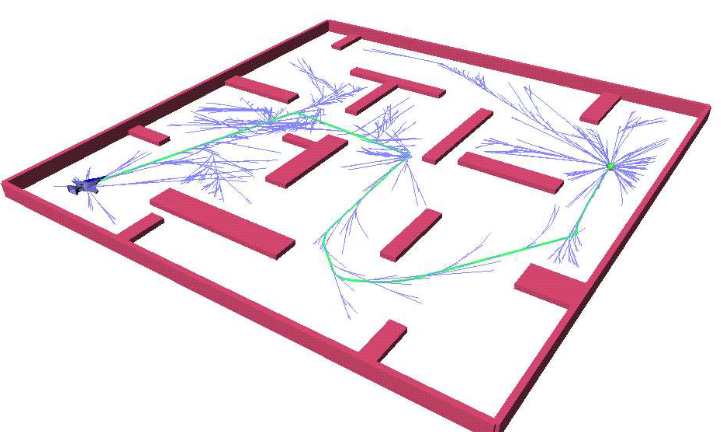
\includegraphics[scale=0.5]{images/rrt1.png}
    \caption{RRTs of 13,600 nodes for the planar body with unilateral thrusters that allow it to rotate freely but translate only in the forward direction. \cite{lavalle2001randomized}}
\end{figure}

The implement of the RRT algorithm in the C++ programming language is given in the code snippet below:

\begin{lstlisting}
// RRT.cpp
#include <iostream>
#include <vector>
#include <cmath>
#include <random>

struct Node {
    double x;
    double y;
    Node* parent;

    Node(double x_val, double y_val, Node* parent_node) {
        x = x_val;
        y = y_val;
        parent = parent_node;
    }
};

double distance(Node* node1, Node* node2) {
    double dx = node1->x - node2->x;
    double dy = node1->y - node2->y;
    return std::sqrt(dx*dx + dy*dy);
}

Node* generateRandomNode(double max_x, double max_y) {
    std::random_device rd;
    std::mt19937 gen(rd());
    std::uniform_real_distribution<double> dist_x(0.0, max_x);
    std::uniform_real_distribution<double> dist_y(0.0, max_y);

    double x = dist_x(gen);
    double y = dist_y(gen);

    return new Node(x, y, nullptr);
}

Node* findNearestNode(std::vector<Node*>& tree, Node* random_node) {
    Node* nearest_node = nullptr;
    double min_distance = std::numeric_limits<double>::max();

    for (Node* node : tree) {
        double dist = distance(node, random_node);
        if (dist < min_distance) {
            min_distance = dist;
            nearest_node = node;
        }
    }

    return nearest_node;
}

Node* steer(Node* nearest_node, Node* random_node, double max_step) {
    double dist = distance(nearest_node, random_node);
    if (dist <= max_step) {
        return random_node;
    } else {
        double theta = std::atan2(random_node->y - nearest_node->y, random_node->x - nearest_node->x);
        double new_x = nearest_node->x + max_step * std::cos(theta);
        double new_y = nearest_node->y + max_step * std::sin(theta);
        return new Node(new_x, new_y, nearest_node);
    }
}

bool isCollisionFree(Node* node) {
    // Check collision with obstacles or environment constraints
    // Implement your collision checking logic here
    return true; // Return true if node is collision-free
}

std::vector<Node*> buildRRT(double start_x, double start_y, double goal_x, double goal_y, double max_x, double max_y, int max_iterations, double max_step) {
    std::vector<Node*> tree;
    Node* start_node = new Node(start_x, start_y, nullptr);
    tree.push_back(start_node);

    for (int i = 0; i < max_iterations; i++) {
        Node* random_node = generateRandomNode(max_x, max_y);
        Node* nearest_node = findNearestNode(tree, random_node);
        Node* new_node = steer(nearest_node, random_node, max_step);

        if (isCollisionFree(new_node)) {
            tree.push_back(new_node);

            // Check if the goal is reached
            if (distance(new_node, goal_node) <= max_step) {
                Node* goal_node = new Node(goal_x, goal_y, new_node);
                tree.push_back(goal_node);
                return tree; // Path found
            }
        }
    }

    return tree; // Path not found
}

int main() {
    double start_x = 0.0;
    double start_y = 0.0;
    double goal_x = 5.0;
    double goal_y = 5.0;
    double max_x = 10.0;
    double max_y = 10.0;
    int max_iterations = 1000;
    double max_step = 0.5;

    std::vector<Node*> rrt_tree = buildRRT(start_x, start_y, goal_x, goal_y, max_x, max_y, max_iterations, max_step);

    // Print the path if it exists
    if (rrt_tree.size() > 0) {
        Node* current_node = rrt_tree.back();
        while (current_node != nullptr) {
            std::cout << "(" << current_node->x << ", " << current_node->y << ")" << std::endl;
            current_node = current_node->parent;
        }
    } else {
        std::cout << "Path not found!" << std::endl;
    }

    // Cleanup: Delete allocated nodes
    for (Node* node : rrt_tree) {
        delete node;
    }

    return 0;
}

\end{lstlisting}

Since cost optimality is always needed for the any robot motion planning algorithm, many variant has been improvised to improve more on the effectiveness of the RRT algorithm, and computational time has also been reduced with the new algorithms like RRT*, RRT*-smart, RRT-plus, etc.

In conclusion, it has been show that the topological complexity that is the optimality of an algorithm is very important in the designing of motion planner for a robot and this also it also takes into consideration the configuration space, the obtacle space, etc, and the constraints on the paths such as weather condition, land structure, warehouse arrangments, etc presents in a robot workspace.

